\documentclass[a4paper]{article}
\usepackage{import}
\usepackage{graphicx}
\usepackage{float}
\usepackage{pgfplots}
\usepackage{listings}
\usepackage{enumitem}
\usepackage{textcomp}
\usepackage{tikz}
\usetikzlibrary{decorations.pathreplacing} % for angle arc
\usetikzlibrary{angles, quotes, calc, positioning, trees} % for drawing angles
\pgfplotsset{compat=1.18,width=10cm}
\usepackage{tikz-cd}
\usepackage{booktabs}
\usepackage{cancel}
\usepackage{amsmath}
\usepackage{minted}
\usepackage{csquotes}
\usepackage{gensymb}
\usepackage{forest}
\usepackage{amsthm}
\usepackage{amssymb}
\usepackage{fontawesome} 
\usepackage{varwidth}
\usepackage{pgfplots}
\usepackage{lipsum}
\usepackage{mdframed} 
\usepackage{color}   
\usepackage{hyperref}
\newmdtheoremenv{theo}{Theorem}
\usepackage{mathtools}
\DeclarePairedDelimiter\ceil{\lceil}{\rceil}
\DeclarePairedDelimiter\floor{\lfloor}{\rfloor}

\hypersetup{
    colorlinks=true, %set true if you want colored links
    linktoc=all,     %set to all if you want both sections and subsections linked
    linkcolor=black,  %choose some color if you want links to stand out
}

% Define theorem styles
\newtheorem{theorem}{Theorem}[section]    % Theorems numbered within sections
\newtheorem{lemma}[theorem]{Lemma}        % Lemmas use the same counter as theorems
\newtheorem{corollary}[theorem]{Corollary} % Corollaries use the same counter as theorems
\newtheorem{proposition}[theorem]{Proposition} % Proposition uses the same counter
\newtheorem{property}[theorem]{Property}
\theoremstyle{definition}
\newtheorem{definition}[theorem]{Definition} % Now uses the same counter as theorems


% Remark-style theorem
\theoremstyle{remark}
\newtheorem{remark}[theorem]{Remark}

% Boxed environment for theorems
\newmdenv[
  linewidth=0.8pt,
  roundcorner=5pt,
  linecolor=black,
  backgroundcolor=white!5,
  skipabove=\baselineskip,
  skipbelow=\baselineskip,
  innerleftmargin=10pt,
  innerrightmargin=10pt,
  innertopmargin=5pt,
  innerbottommargin=5pt
]{thmbox}

% Custom proof environment (also boxed)
\renewenvironment{proof}[1][Proof]{%
  \begin{mdframed}[linewidth=0.8pt, roundcorner=5pt, linecolor=black, skipabove=\baselineskip, skipbelow=\baselineskip, innertopmargin=5pt, innerbottommargin=5pt]%
  \noindent\textbf{#1. }%
}{%
  \end{mdframed}%
}

% Redefine theorem environments to use thmbox
\let\oldtheorem\theorem
\renewenvironment{theorem}{\begin{thmbox}\begin{oldtheorem}}{\end{oldtheorem}\end{thmbox}}

\let\oldlemma\lemma
\renewenvironment{lemma}{\begin{thmbox}\begin{oldlemma}}{\end{oldlemma}\end{thmbox}}

\let\oldcorollary\corollary
\renewenvironment{corollary}{\begin{thmbox}\begin{oldcorollary}}{\end{oldcorollary}\end{thmbox}}

\let\oldproposition\proposition
\renewenvironment{proposition}{\begin{thmbox}\begin{oldproposition}}{\end{oldproposition}\end{thmbox}}

\let\oldproperty\property
  \renewenvironment{property}{\begin{oldproperty}}{\end{oldproperty}}


% Reference shortcuts
\newcommand{\thmref}[1]{Theorem~\ref{#1}}
\newcommand{\lemref}[1]{Lemma~\ref{#1}}
\newcommand{\corref}[1]{Corollary~\ref{#1}}
\newcommand{\propref}[1]{Property~\ref{#1}} 

% To customize QED symbol
\renewcommand{\qedsymbol}{$\blacksquare$}

\usetikzlibrary{decorations.pathreplacing} % for angle arc
\usetikzlibrary{angles, quotes, calc} % for drawing angles

\usepackage{color}   %May be necessary if you want to color links
\usepackage{hyperref}
\hypersetup{
    colorlinks=true, %set true if you want colored links
    linktoc=all,     %set to all if you want both sections and subsections linked
    linkcolor=black,  %choose some color if you want links to stand out
}

\usepackage{xcolor}
\usepackage[most]{tcolorbox}


% Define a custom tcolorbox environment for examples
\newtcolorbox{examplebox}[2][]{
  colback=blue!5!white,
  colframe=blue!30!black,
  title=#2,
  boxrule=0mm,
  fonttitle=\bfseries,
  width=\textwidth,
  breakable,
  #1
}

\newtcolorbox{definizione}[2] {
  colback=green!5!white,
  colframe=green!30!black,
  title=#2,
  boxrule=0mm,
  fonttitle=\bfseries,
  width=\textwidth,
  breakable,
  #1
}

\definecolor{codegreen}{rgb}{0,0.6,0}
\definecolor{codegray}{rgb}{0.5,0.5,0.5}
\definecolor{codepurple}{rgb}{0.58,0,0.82}
\definecolor{backcolour}{rgb}{0.95,0.95,0.92}

\lstdefinestyle{mystyle}{
    backgroundcolor=\color{backcolour},   
    commentstyle=\color{codegreen},
    keywordstyle=\color{magenta},
    numberstyle=\tiny\color{codegray},
    stringstyle=\color{codepurple},
    basicstyle=\ttfamily\footnotesize,
    breakatwhitespace=false,         
    breaklines=true,                 
    captionpos=b,                    
    keepspaces=true,                 
    numbers=left,                    
    numbersep=5pt,                  
    showspaces=false,                
    showstringspaces=false,
    showtabs=false,                  
    tabsize=2
}

\lstset{style=mystyle}

\makeatletter
\renewcommand*\env@matrix[1][*\c@MaxMatrixCols c]{%
  \hskip -\arraycolsep
  \let\@ifnextchar\new@ifnextchar
  \array{#1}}
\makeatother

\title{Operating Systems - Paper on Input/Output Devices}
\author{SETU - South East Technological University\\Imbriani Paolo - W20114452\\Professor Micheal McMahon}

\begin{document}

\begin{figure}
    \centering
    
\includegraphics[width=0.6\textwidth]{SETU.png}
    \label{fig:centered-image}
\end{figure}

\maketitle 

\begin{abstract}
    Input/Output (I/O) systems are the fundamentals on how the processing core of a computer interact with the outside world. This dissertation wants to analyze the architecture, design principles, and 
    performance considerations of I/O systems. Emphasis is placed on both hardware components
     (such as device controllers, interfaces, and direct memory access) and software mechanisms 
     (including device drivers, I/O scheduling, and caching). Finally, emerging trends—such as 
     high-speed interfaces, virtualization challenges, and the integration of AI in I/O management—are 
     discussed, highlighting the evolving nature of these systems in the context of modern computing.
\end{abstract}


\pagebreak

\tableofcontents

\pagebreak

\section*{Introduction}

Input/Output systems, simply put, enable computers to interact with its environment.
They connect the central processing unit (CPU) with various peripheral devices—ranging from 
keyboards and displays, to storage systems and network interfaces. As modern computing demands 
increased speed, efficiency, and reliability, the design and management of I/O systems have become 
critically important. This paper examines the fundamental components of I/O systems and their history, their role 
within operating systems, and the impact of emerging technologies on future developments.

\begin{figure}[H]
    \centering
    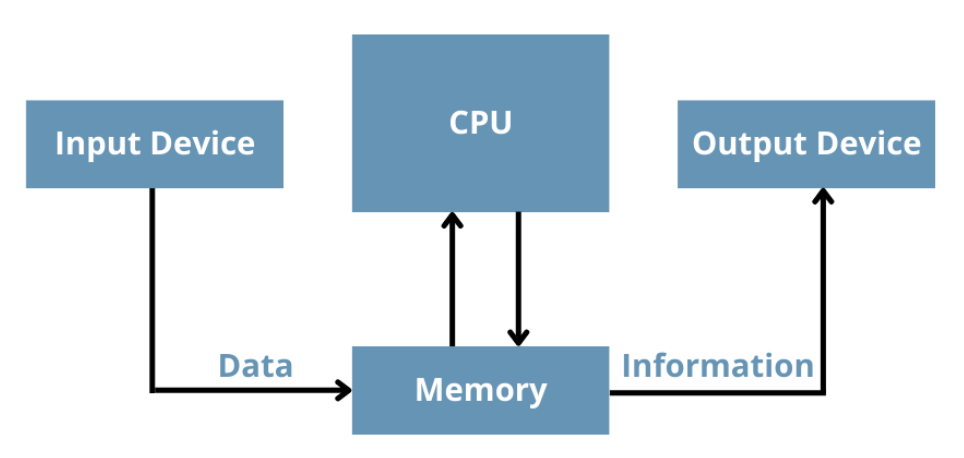
\includegraphics[width=0.6\textwidth]{IO.png}
    \caption{Flow of data between inputs/outputs, memory and processing units.}
\end{figure}

For instance: a user wants to type a document on a computer.
In this scenario, the keyboard would be the input device. 
By pressing letter, number, and symbol keys, a user can submit data and
instructions to the computer. Each key is transformed into a \textit{binary number} that the
CPU can \textit{interpret and recognize}. This is stored in the system’s memory and transferred 
to the CPU to perform its calculations to provide an output result. 
Then, this is information is displayed in the output device, such as a monitor.



\section{Overview of I/O Systems}

I/O systems connects both hardware and software elements that coordinate data 
exchange between the CPU and peripheral devices. Key functions include:

\begin{itemize}
    \item \textbf{Data Transfer}: Moving data to and from peripherals.
    \item \textbf{Control}: Managing device operations and status.
    \item \textbf{Error Handling}: Detecting and recovering from faults.
\end{itemize}
Efficient I/O systems must balance competing requirements such as throughput, latency, 
and resource utilization to ensure seamless operation [1].


\section{I/O Hardware Components}

The hardware side of I/O systems involves several critical components:

\begin{itemize}
    \item \textbf{Device Controllers}: Interface between the CPU and peripheral devices.
    \item \textbf{Interfaces}: Connect controllers to devices via buses or networks.
    \item \textbf{Direct Memory Access (DMA)}: Enables devices to access memory without CPU intervention.
\end{itemize}
A general-purpose computer system consists of CPUs and multiple device
controllers that are connected through a \textit{common bus}.

\begin{figure}[H]
    \centering
    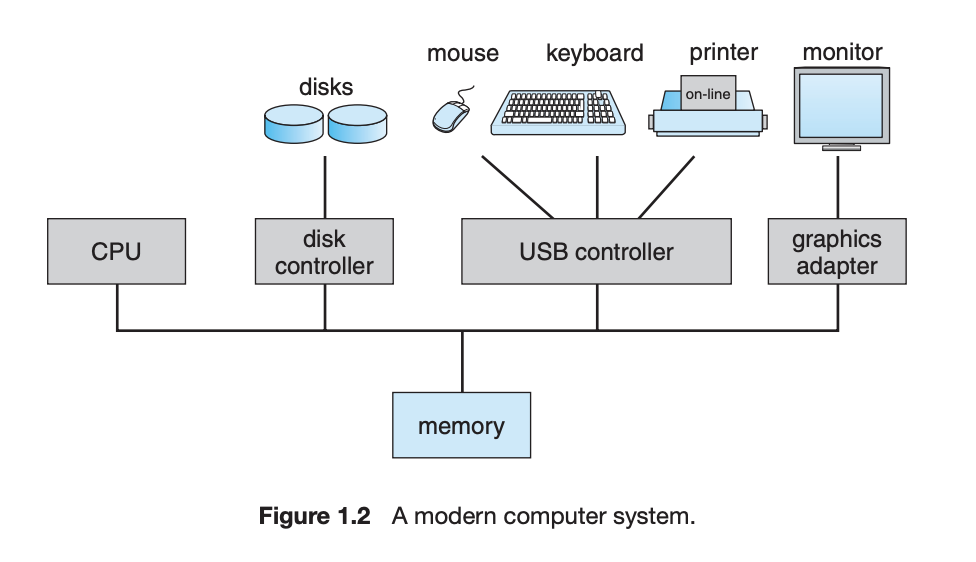
\includegraphics[width=1\textwidth]{Amod.png}
\end{figure}

\subsection{Device Controllers}

Device controllers serve as a bridge between the processing unit and peripheral devices. They interpret the commands issued by 
the operating system and manage the specifics of data transfer. Each device controller
is in charge of a specific type of device. Depending on the controller, more
than one device may be attached.  A device controller maintains some local buffer storage and a set of special-purpose
registers. The device controller is responsible for moving the data between
the peripheral devices that it controls and its local buffer storage. Typically,
operating systems have a device driver for each device controller. This device
driver understands the device controller and provides the rest of the operating
system with a uniform interface to the device.
\\
\vspace{1em}

\noindent
Let's say we want to start an I/O operation. What does the process look like?

\begin{enumerate}
    \item The device driver loads the appropriate registers
    within the device controller.
    \item The device controller, in turn, examines the
    contents of these registers to determine what action to take (such as “read
    a character from the keyboard”).
    \item The controller starts the transfer of data from
    the device to its local buffer. 
    \item Once the transfer of data is complete, the device
    controller informs the device driver via an interrupt that it has finished its
    operation. s
    \item The device driver then returns control to the operating system,
    possibly returning the data or a pointer to the data if the operation was a read.
    For other operations, the device driver returns status information. [1]
\end{enumerate}

\subsection{Interfaces and Buses}

Communication between the CPU and peripherals is facilitated by buses and interfaces. Here some examples:

\begin{itemize}
    \item Peripheral Component Interconnect Express (PCIe): High-speed interface for connecting devices to the CPU.
    \item Universal Serial Bus (USB): Widely used interface for connecting peripherals to computers.
    \item Serial ATA (SATA): Interface for connecting storage devices to the motherboard.
\end{itemize}
These interfaces are widely spread in the world and now standardized in the world of communication protocols and ensure that data is transferred efficienctly and reliably.

\subsection{Direct Memory Access (DMA)}

When CPU need to fetch an instruction or data from memory, it always controls the status of the device and that could be done using \textbf{interrupts} that is a hardware signals 
that interrupts the normal flow of execution only when the device is ready. But to
 transfer large amounts of data from an input/output device to memory, it is
not advisable to use interrupts because it would be a waste of resources. DMA is used, which 
is a device that allows data to be transferred from memory to the input/output device without passing 
through the CPU. [1] [2]


\begin{figure}[H]
    \centering
    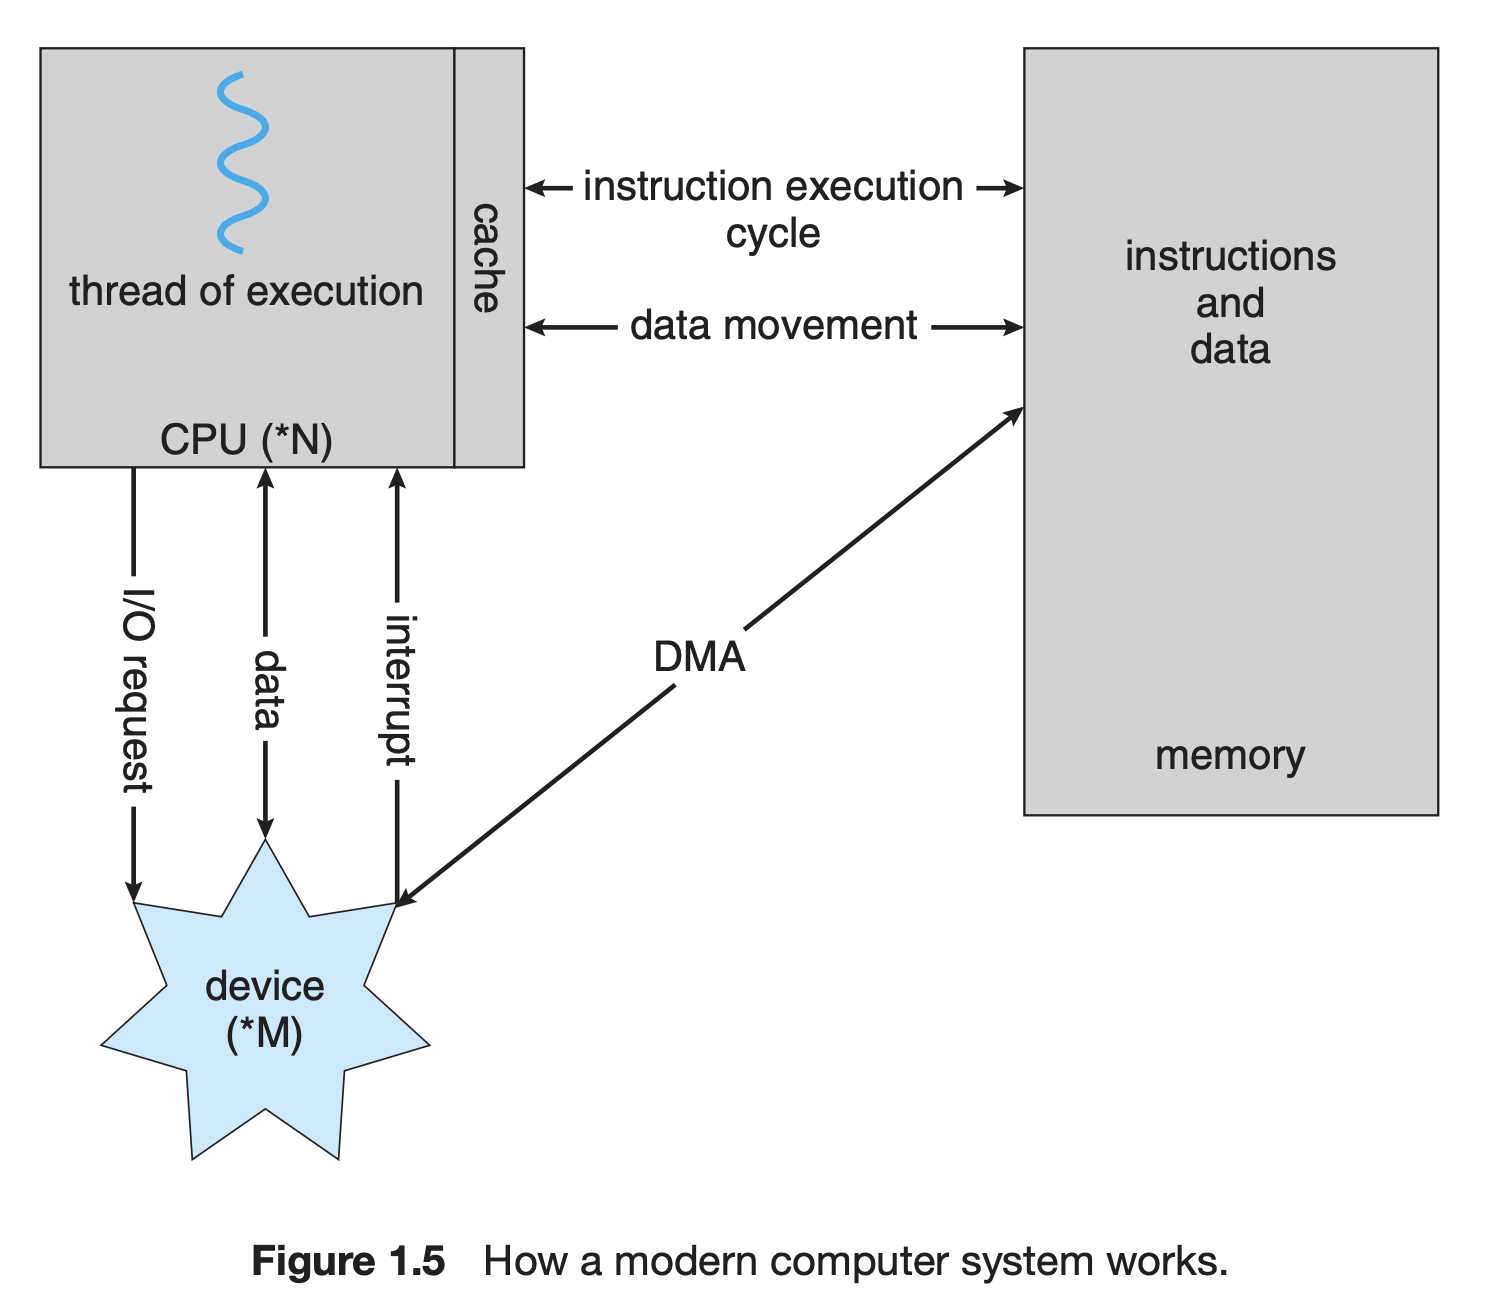
\includegraphics[width=0.6\textwidth]{DMA.png}
\end{figure}

\section{I/O Software and Operating System Support}

The software layer of I/O systems is very important since it has to manage hardware resources effectively and efficienctly.


\begin{thebibliography}{9}
    \bibitem{texbook}
    Silberschatz A, Galvin PG, Gagne G. Operating System Concepts. 9th ed. Wiley; 2013.
    \bibitem{texbook}
    Hennessy J, Patterson D. Computer Architecture: A Quantitative Approach. 5th ed. Morgan Kaufmann; 2011.
\end{thebibliography}






\end{document}